%%%%%%%%%%%%%%%%%%%%%%%%%%%%%%%%%%%%%%%%%%%%%%%%%%%%%%%%%%%%%%%%%%%%%%%%%%%%%%%%%%%%%%%%%%%%%%%%%%%%
% Project Requirements Specification Report
% Authors: Michael Galliers and James Miller
% Course: CSC 440
%%%%%%%%%%%%%%%%%%%%%%%%%%%%%%%%%%%%%%%%%%%%%%%%%%%%%%%%%%%%%%%%%%%%%%%%%%%%%%%%%%%%%%%%%%%%%%%%%%%%

\documentclass[12pt]{article}
\usepackage[utf8]{inputenc}
\usepackage{graphicx}
\usepackage{float}
\usepackage{tocloft}

% Document configuration

% Section numbering
\renewcommand \thesection{\Roman{section}}
\renewcommand \thesubsection{\arabic{section}.\arabic{subsection}}

% Environment config for requirements
%  - Configures formatting of the section heading and numbered, nested lists
\newenvironment{requirement}[1]
{
    % Format requirement sections (R1. ...)
    \renewcommand{\thesubsubsection}{R\arabic{subsubsection}.}
    % Format nested, numbered lists (1.1, 1.1.1, 1.1.1.1, ...)
    \renewcommand{\labelenumi}{
        \arabic{subsubsection}.\arabic{enumi}
    }
    \renewcommand{\labelenumii}{
        \arabic{subsubsection}.\arabic{enumi}.\arabic{enumii}
    }
    \renewcommand{\labelenumiii}{
        \arabic{subsubsection}.\arabic{enumi}.\arabic{enumii}.\arabic{enumiii}
    }
    \renewcommand{\labelenumiv}{
        \arabic{subsubsection}.\arabic{enumi}.\arabic{enumii}.\arabic{enumiii}.\arabic{enumiv}
    }
    % Create the subsubsection for the requirement
    \subsubsection{#1}
}
{}


% Set path to all graphics
\graphicspath{{figures/}}

% Do paragraph indenting after section tags
\usepackage{indentfirst}

% Adjust space between numbers and headings in table of contents
\addtolength{\cftsecnumwidth}{12pt}
\addtolength{\cftsubsubsecnumwidth}{-10pt}


\author{Michael Galliers and James Miller}
\title{CSC 440 - Requirements Specification Report}


\begin{document}

\begin{titlepage}
\maketitle
\end{titlepage}

\newpage
    \tableofcontents
\newpage

\section{Introduction}
\subsection{Problem Statement}

\subsection{Proposal}

\section{System Description}

\section{System Requirements}
\subsection{Functional Requirements}
\begin{requirement}{The system shall..1}


\begin{enumerate}
    \item Test item 1
    \item Test item 2
    \begin{enumerate}
        \item Test item 1.1
        \item Test item 1.2
        \begin{enumerate}
            \item Test item 1.1.1
            \item Test item 1.1.2
            \begin{enumerate}
                \item Test item 1.1.1.1
                \item Test item 1.1.1.2
            \end{enumerate}
        \end{enumerate}
    \end{enumerate}
\end{enumerate}


\end{requirement}

\begin{requirement}{The system shall..2}


\begin{enumerate}
    \item Test item 1
    \item Test item 2
    \begin{enumerate}
        \item Test item 1.1
        \item Test item 1.2
        \begin{enumerate}
            \item Test item 1.1.1
            \item Test item 1.1.2
            \begin{enumerate}
                \item Test item 1.1.1.1
                \item Test item 1.1.1.2
            \end{enumerate}
        \end{enumerate}
    \end{enumerate}
\end{enumerate}


\end{requirement}

\subsection{Non-functional Requirements}

\subsection{Domain Requirements}

\section{Use-case Diagram}

\section{Class Diagram}

\section{Sequence Diagrams}

\section{State Diagram}

\section{Activity Diagrams}

\section{Database Design}

\begin{figure}[p!]
  \subsection{ER Schema}
  \centering
  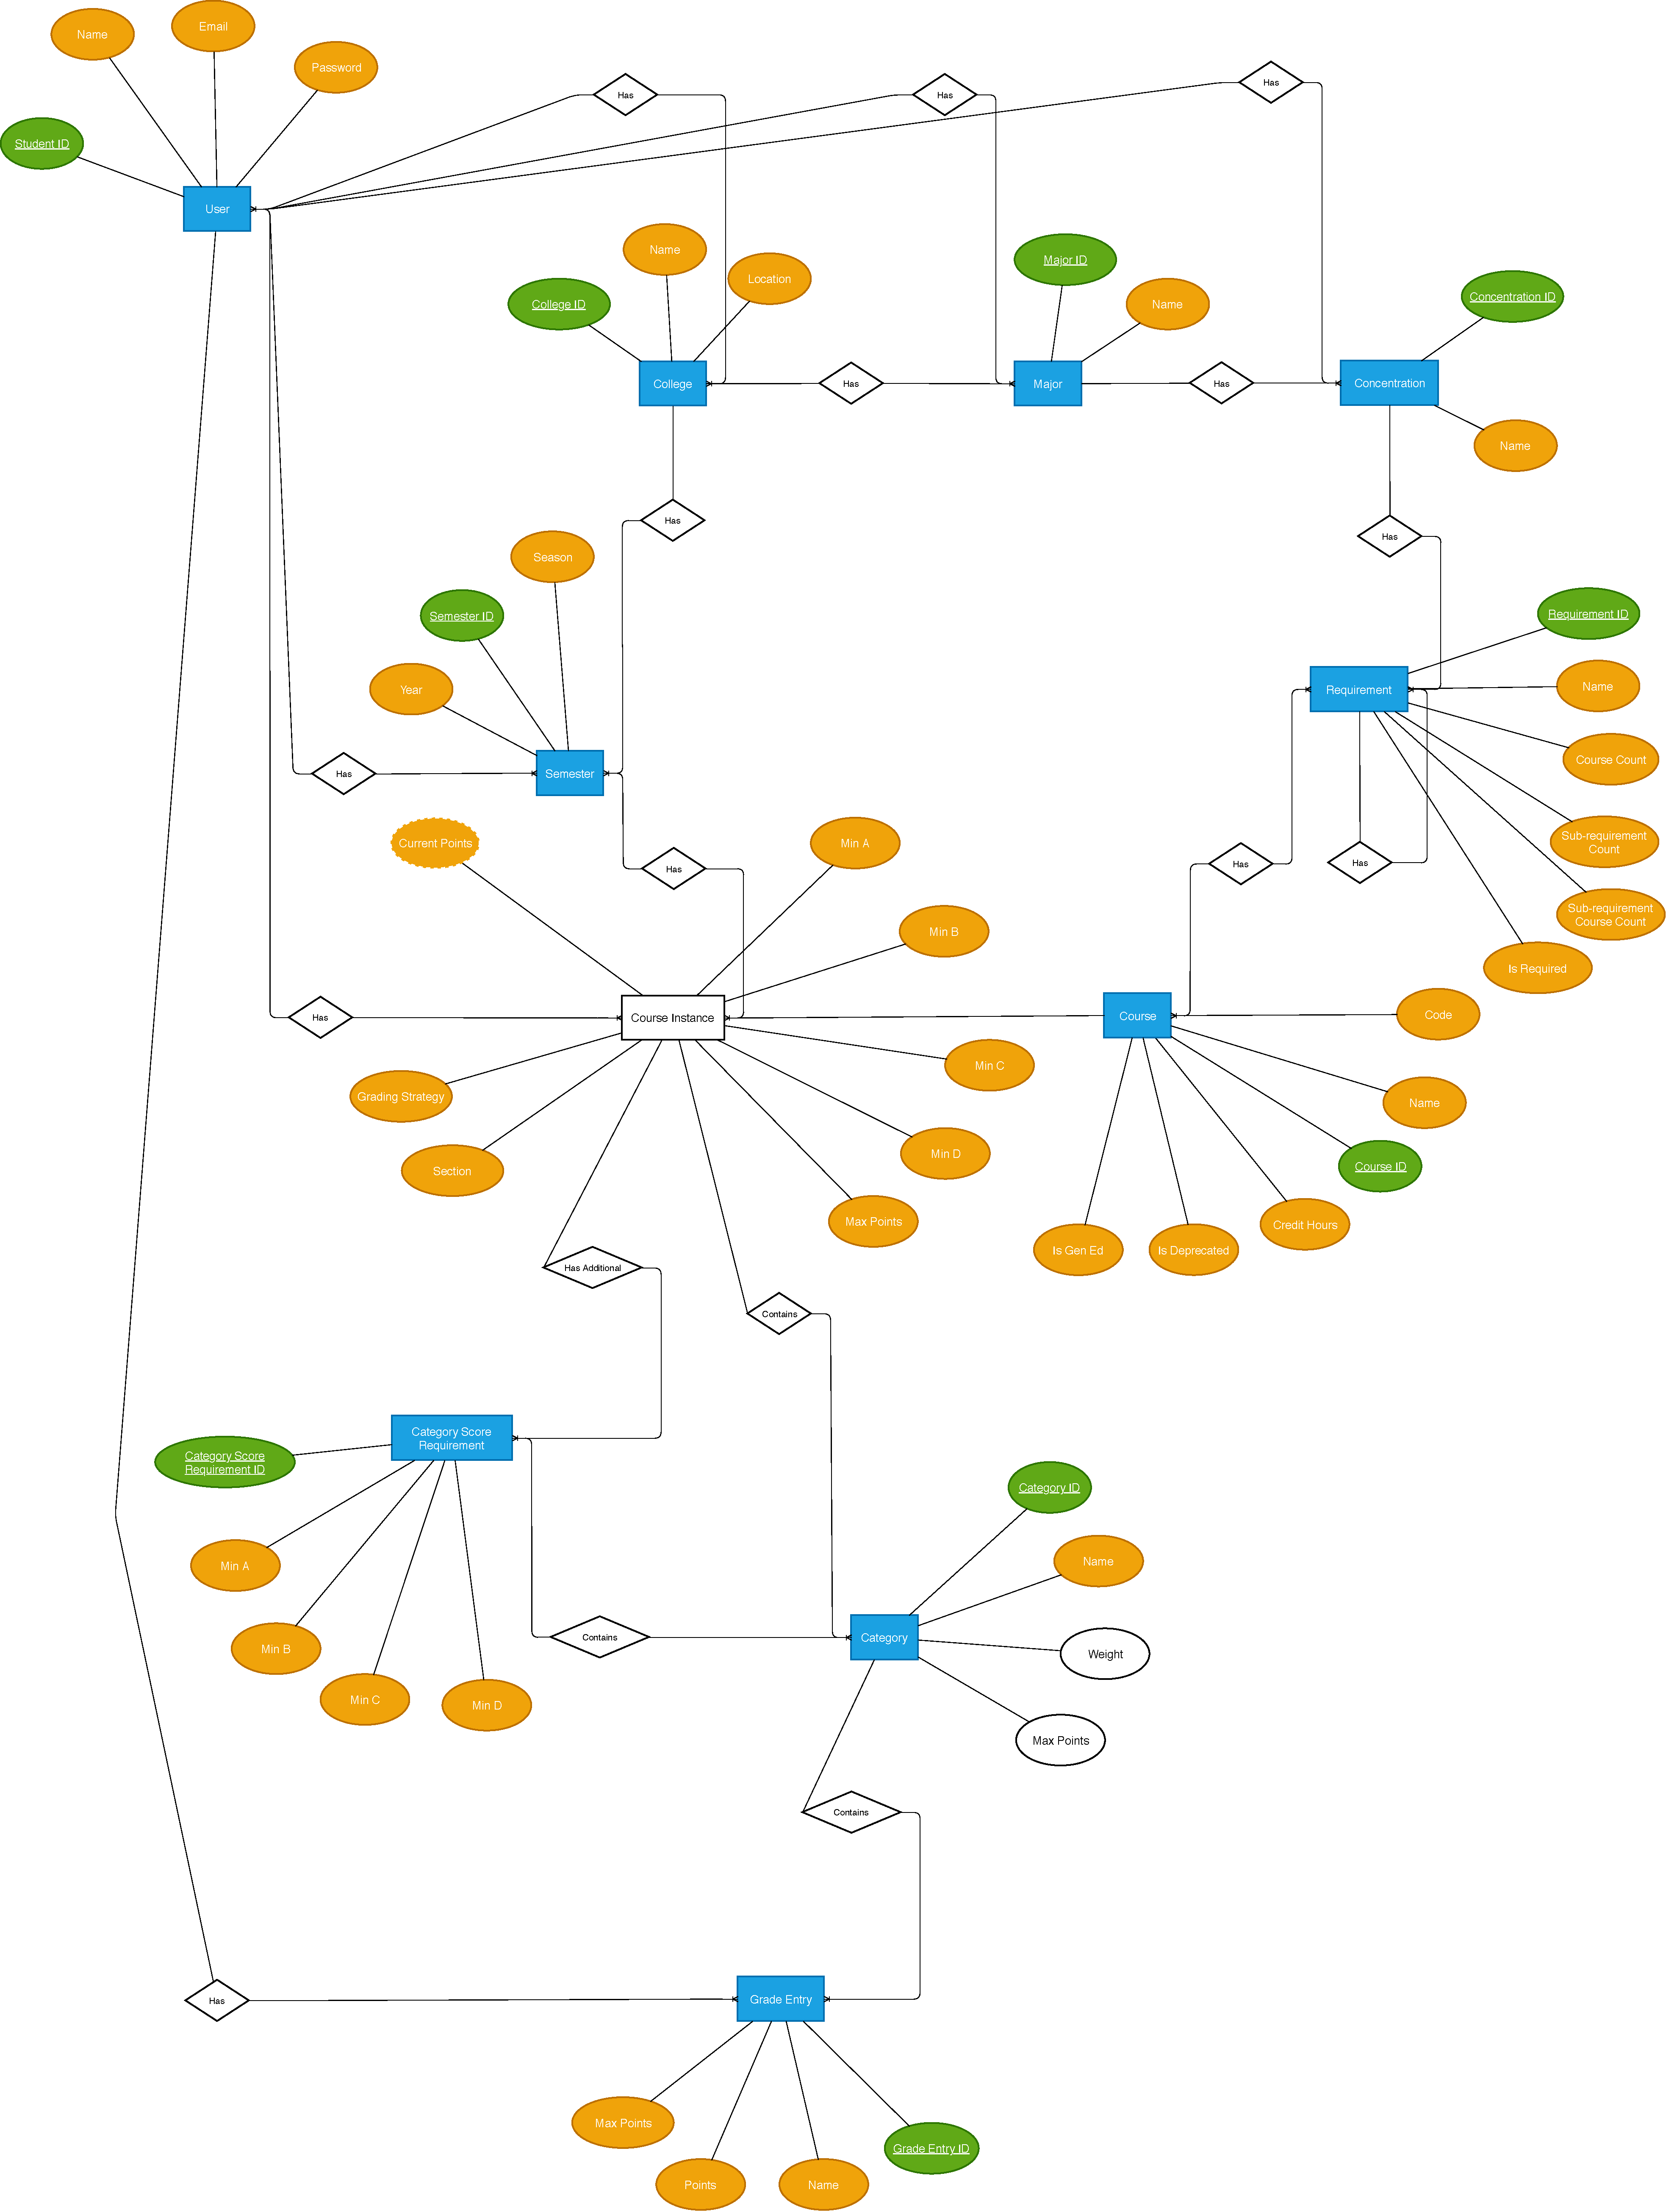
\includegraphics[width=\linewidth]{database_erd.pdf}
  \caption{Database ERD}
\end{figure}

\clearpage

\subsection{Table Schema}

\section{Conclusion}

\section{Dictionary}
\begin{itemize}
    \item \textbf{Semester}: A single semester of education consisting of courses. Each semester can
    be associated with a different educational institution; consistency is not required.
    \item \textbf{Course}: Any educational course/class occurring within a particular semester.
    \item \textbf{Section}: An equally weighted or logically grouped collection of material within a
    particular course (e.g. Homework, Tests, etc.).
    \item \textbf{Grade Entry}: A graded piece of material associated with a particular section 
    (e.g. Homework 2, Exam 1, etc.).
\end{itemize}

\end{document}
